%   ##
%
%   Band VIII, 3 N.~??A10.4
%   Signatur/Tex-Datei: LH_35_09_15_012-013
%   RK-Nr. 41152 [Teil 4]
%   Überschrift: Tentaminum de chordarum tensione scheda quarta
%   Datierung: 1680.12.00
%   WZ: (keins)
%.  SZ: (keins)
%.  Bilddateien (PDF): LH_35_09_15_012-013_d1; LH_35_09_15_012-013_d2; LH_35_09_15_012-013_d3a; LH_35_09_15_012-013_d3b (insgesamt vier)
%
%
\begin{ledgroupsized}[r]{120mm}
\footnotesize
\pstart
\noindent\textbf{Überlieferung:}
\pend
\end{ledgroupsized}
\begin{ledgroupsized}[r]{114mm}
\footnotesize
\pstart \parindent -6mm
\makebox[6mm][l]{\textit{L}}%
Aufzeichnung: LH XXXV 9, 15 Bl. 12\textendash13.
Ein Bogen 4\textsuperscript{o}.
Vier meist einspaltig beschriebene Seiten.
N.~8\textsubscript{4} setzt den Text von N.~8\textsubscript{3} fort.
% Der Text von N.~??A10\textsubscript{4} wird in N.~??A10\textsubscript{5} fortgesetzt.
% Zahlreiche Streichungen, Ergänzungen und Ersetzungen.
Am oberen Rand von Bl.~13~v\textsuperscript{o} gestrichenes Satzfragment von Leibnizens Hand:
\textit{Sunt enim ut celeritates}.
Die Textträger von N.~8\textsubscript{4} und N.~8\textsubscript{6} bildeten ursprünglich einen Folio-Bogen.
% Kein Wasserzeichen.
\pend
\end{ledgroupsized}
%
%
\vspace{4mm}% Vorläufig verkleinert
\pstart%
\count\Bfootins=1200
\count\Afootins=1200
\count\Cfootins=1200
\normalsize%
\noindent%
%
\lbrack12~r\textsuperscript{o}\rbrack% Blatt 12r
%
\pend%
% \vspace*{0.5em}
% Überschrift
\pstart%
\centering%
Tentaminum\protect\index{Sachverzeichnis}{tentamen}
de chordarum Tensione\protect\index{Sachverzeichnis}{tensio chordae}\\
Scheda\protect\index{Sachverzeichnis}{scheda} 4\textsuperscript{ta}
Xb. \edlabel{LH_35_09_15_012r_anfang-1}1680
\edtext{}{{%
\xxref{LH_35_09_15_012r_anfang-1}{LH_35_09_15_012r_anfang-2}}{%
\lemma{1680}\Bfootnote{%
\textit{(1)}~Superest igitur ut definiamus, quaenam
\textit{(a)}~sint te
\textit{(b)}~sit ratio
\textit{(aa)}~vibra
\textit{(bb)}~temporum quibus duae chordae similes et aequales, sed diverso modo tensae vibrant. Sane si
\textit{(2)}~Chordae\protect\index{Sachverzeichnis}{chorda tensa}
\textit{(a)}~po
\textit{(b)}~cum
\textit{(3)}~Cum motus chordarum%
~\textit{L}}}}
\pend%
\vspace{0.5em}%
%
\pstart%
\noindent%
Cum\edlabel{LH_35_09_15_012r_utsubduplrt-3}
motus chordarum\protect\index{Sachverzeichnis}{motus chordae}%
\edlabel{LH_35_09_15_012r_anfang-2}
se restituentium sit acceleratus,\protect\index{Sachverzeichnis}{motus acceleratus}
si ponerentur incrementa\protect\index{Sachverzeichnis}{incrementum motus}
quovis momento temporis\protect\index{Sachverzeichnis}{momentum temporis} esse eadem,
ut in gravibus\protect\index{Sachverzeichnis}{grave descendens}
\edtext{descendentibus,
videndum quid sit futurum.%
\edlabel{LH_35_09_15_012r_utsubduplrt-4}}{%
\lemma{descendentibus,}\Bfootnote{%
\textit{(1)}~manifeste forent tempora in ratione tensionum subduplicata, quod sic ostendo.
\textit{(2)}~videndum quid sit futurum.%
~\textit{L}}}%
\pend
% \newpage%
% \vspace{1.5em}%
%
%
\pstart%
Sint duae chordae
\edtext{$AB$ et $LR$}{%
\lemma{$AB$}\Bfootnote{%
\hspace{-0,5mm}et
\textit{(1)}~$CD$
\textit{(2)}~$LR$%
~\textit{L}}}
aequales et similes et hoc uno differentes
quod una magis tensa est quam altera\protect\index{Sachverzeichnis}{chorda tensa}
et pulsentur ambae eodem modo,
ita
\edtext{ut $AB$ pulsata\protect\index{Sachverzeichnis}{chorda pulsata}}{%
\lemma{ut}\Bfootnote{%
\hspace{-0,5mm}$AB$
\textit{(1)}~tensa
\textit{(2)}~pulsata%
~\textit{L}}}
adducatur in
\edtext{$AEB$ et $LR$}{%
\lemma{$AEB$}\Bfootnote{%
\hspace{-0,5mm}et
\textit{(1)}~$CD$
\textit{(2)}~$LR$%
~\textit{L}}}
pulsata\protect\index{Sachverzeichnis}{chorda pulsata} in
\edtext{\lbrack$LFR$\rbrack.}{%
\lemma{$CFD$}\Bfootnote{\textit{L~ändert Hrsg.}}}
Cumque $AEB$ congruat
\edtext{ipsi $LFR$}{%
\lemma{ipsi}\Bfootnote{%
\textit{(1)}~$CFD$
\textit{(2)}~$LFR$%
~\textit{L}}}
omniaque conveniant praeter tempus,\protect\index{Sachverzeichnis}{tempus restitutionis}
necesse est enim magis tensam celerius restitui;
hinc
\edtext{ponatur tempus quo chorda minus tensa\protect\index{Sachverzeichnis}{chorda tensa}}{%
\lemma{ponatur}\Bfootnote{%
\textit{(1)}~chordae
\textit{(2)}~tempus quo chorda
\textit{(a)}~magis tensa s
\textit{(b)}~minus tensa%
~\textit{L}}}
\hspace{0.1mm}$AB$\hspace{0.2mm} restituitur\hspace{0.1mm} esse\hspace{0.2mm}
\edtext{ut $HK$}{%
\lemma{ut $HK$}\Cfootnote{%
Siehe das Diagramm \lbrack\textit{Fig.~2}\rbrack\ auf S.~\pageref{LH_35_09_15_012r_Fig.2}.}}
%
eique\hspace{0.2mm} applicari\hspace{0.1mm} spatia\protect\index{Sachverzeichnis}{spatium percursum}\hspace{0.2mm}
quolibet\hspace{0.05mm} temporis
% !!!!! Getrixt: Folgende Cfootnote hängt eigentlich an das Diagramm Fig. 1. !!!!!
\edtext{}{%
\lemma{\hspace*{1,6mm}\lbrack\textit{Fig.~1}\rbrack}\killnumber%
\Cfootnote{Die Saite $LR$ hieß ursprünglich $CD.$}}
%
\pend%
%
%
 \vspace{1em}%
 \centerline{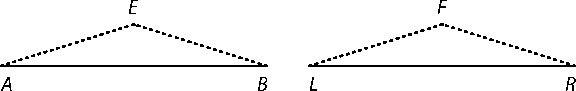
\includegraphics[width=0.77\textwidth]{gesamttex/edit_VIII,3/images/LH_35_09_15_012-013_d1.pdf}}%
 \vspace{0.5em}
 \centerline{\lbrack\textit{Fig.~1}\rbrack}%
\newpage
\count\Bfootins=1000
\count\Afootins=900
\count\Cfootins=1000
\pstart 
\noindent
\makebox[1.0\textwidth][s]{momento\protect\index{Sachverzeichnis}{momentum temporis} percursa,
patet crescentes uniformiter celeritates
\edtext{acquisitas\protect\index{Sachverzeichnis}{celeritas acquisita}}{%
\lemma{acquisitas}\Bfootnote{\textit{erg.~L}}}
ex hypotesi,\protect\index{Sachverzeichnis}{hypothesis}}
\newline
\makebox[1.0\textwidth][s]{\edtext{vel}{%
\lemma{vel}\Bfootnote{\textit{erg.~L}}} spatia ab aliquo
\edtext{puncto (ut $E$) quovis temporis momento\protect\index{Sachverzeichnis}{momentum temporis}
successive}{%
\lemma{puncto}\Bfootnote{%
\textit{(1)}~ut $E$
\textit{(2)}~(ut $E$) \lbrack...\rbrack\ momento successive% quovis temporis
~\textit{L}}}
percursa\protect\index{Sachverzeichnis}{spatium percursum}
cres-}
\newline cere ut rectas applicatas triangulo $HKG,$\protect\index{Sachverzeichnis}{triangulum}
\edtext{posito $KG$ respondere ultimo percurso spatio,}{%
\lemma{posito}\Bfootnote{%
\hspace{-0,5mm}$KG$
\textit{(1)}~esse \textbar~ut \textit{erg.}~\textbar\ ultimum percursum spatium,
\textit{(2)}~respondere ultimo percurso spatio,%
~\textit{L}}}
\makebox[1.0\textwidth][s]{vel ultimae celeritati acquisitae\lbrack,\rbrack\protect\index{Sachverzeichnis}{celeritas acquisita}
\edtext{et area trianguli $HKG$ respondebit toto spatio.}{%
\lemma{et}\Bfootnote{%
\hspace{-0,5mm}area \lbrack...\rbrack\ toto spatio \textit{erg.~L}}}
Sit}
\newline
\makebox[1.0\textwidth][s]{jam aliud triangulum $HXY$\protect\index{Sachverzeichnis}{triangulum}
\edtext{pro chorda magis tensa $LR,$\protect\index{Sachverzeichnis}{chorda tensa}}{%
\lemma{pro}\Bfootnote{%
\hspace{-0,5mm}chorda
\textit{(1)}~\textbar~tensa, \textit{streicht Hrsg.}~\textbar\
\textit{(2)}~magis tensa $LR,$%
~\textit{L}}}
sitque
\edtext{\lbrack$HX$\rbrack}{%
\lemma{$VX$}\Bfootnote{%
\textit{L~ändert Hrsg.}}}
%
tempus quo}
\newline
\edtext{chorda $LR$ pulsata\protect\index{Sachverzeichnis}{chorda pulsata}
redit\lbrack,\rbrack\
$XY$ ultima celeritas quaesita\protect\index{Sachverzeichnis}{celeritas quaesita}}{%
\lemma{chorda}\Bfootnote{%
\hspace{-0,5mm}$LR$
\textit{(1)}~restituitur
\textit{(2)}~pulsata redit
\textit{(a)}~jamque sint impetus impressi semper dupli
\textit{(b)}~$XY$ ultima celeritas quaesita%
~\textit{L}}}
seu ultimum spatium percursum,\protect\index{Sachverzeichnis}{spatium percursum}
triangulum $HXY$ totum spatium,
cumque sit spatium utrobique
\edtext{idem, necesse est}{%
\lemma{idem,}\Bfootnote{%
\textit{(1)}~seu cum
\textit{(2)}~necesse est%
~\textit{L}}}
triangula\protect\index{Sachverzeichnis}{triangulum} $HXY$ et $HKG$
% <<<<<<<<<<<<<<<<<<<<<<<<<<
\edtext{esse aequalia.
Ergo $\displaystyle HK\!:\!HX \squaredots XY\!:\!KG.$
Jam ipsa $HG$ secet ipsam $XY$ in $V.$
Patet $XV$ esse celeritatem
quam chorda tardior $AB$ quaesivit,
eo tempore $HX$ quo chorda
\lbrack celerior\rbrack\
$LR$ absolvit suam restitutionem.\protect\index{Sachverzeichnis}{restitutio chordae}
Jam celeritates iisdem temporibus quaesitae\protect\index{Sachverzeichnis}{celeritas quaesita}
a diversis chordis sola tensione differentibus,\protect\index{Sachverzeichnis}{tensio chordae}
sunt
\lbrack ut\rbrack\
ipsae tensiones\protect\index{Sachverzeichnis}{tensio chordae}
seu pondera chordis appensa.\protect\index{Sachverzeichnis}{pondus appensum}
Ergo $XV\!:\!XY \,\squaredots$ tens. $AB$ : tens. $LR.$
Jam et $\displaystyle HX\!:\!HK \squaredots XV\!:\!KG$~%
et per sup. $\displaystyle\squaredots\, KG\!:\!XY.$
Ergo $KG$ media proport. inter~$XV,$~$XY.$
%%%%%%%%%%%%%%%%%%%%%%%%%%%%%%%%%%%%%
%Jam $XV$ quad. : 
%\protect\rule[-8mm]{0mm}{12mm}$KG\ \hspace{-6,9mm}\displaystyle\efrac{\phantom{\frac{}{\displaystyle\int}}}{\overbrace{XV, XY}} \hspace{-6,9mm}$ quad.~
%$\squaredots$ $HX$~quad. : $HK$~quad.
%Ergo $XV\!: XY\!\squaredots HX$ quad.~:~$HK$ quad.
%%%%%%%%%%%%%%%%%%%
Jam $XV$ quad. : 
$KG\;\hspace{-6,9mm}$ 
\protect\raisebox{-6mm}{$\displaystyle\overbrace{XV, XY}$}$\hspace{-6,9mm}$ quad. 
$\squaredots$ $HX$~quad. : $HK$~quad.
Ergo $XV\!: XY\!\squaredots HX$ quad.~:~$HK$ quad.
%%%%%%%%%%%%%%%%%%%%%%%%%%%%%%%%%%%%%%%%%%%
Seu\edlabel{LH_35_09_15_012r_utsubduplrt-1}
pondera\protect\index{Sachverzeichnis}{pondus tendens}
vel tensiones\protect\index{Sachverzeichnis}{tensio chordae}
in duplicata ratione vibrationum\protect\index{Sachverzeichnis}{vibratio chordae}
reciproce.}{%
\lemma{esse}\Bfootnote{%
% Ungültige Stufen
\textit{(1)}~aequalia, est autem $XY$ duplum ipsius $KG,$ quia
\textit{(2)}~\textbar~ad $KG$ \textit{streicht Hrsg.}~%
\textbar\ ut tensio nempe impetus ultimus acquisitus unus
\textbar~ad \textit{erg.}~%
\textbar\ alterum, ut impetus primi seu ut tensiones ob incrementa proportionalia.
\textit{(a)}~Ergo
\textit{(aa)}~cum
\textit{(bb)}~necesse est
\textit{(b)}~Et ut
\textit{(c)}~Ergo sequeretur tempora restitutionum esse ut tensiones reciproce. 
% Gültige Stufe
\textit{(3)}~aequalia. Ergo $\displaystyle HK : HX \squaredots\, XY : KG.$
\textit{(a)}~Jam quo tempore, nempe $HX$
\textit{(b)}~Jam ipsa $HG$ \lbrack...\rbrack\ quam chorda
\textit{(aa)}~quaesivit
\textit{(bb)}~tardior $AB$ \lbrack...\rbrack\ $HX$ quo % quaesivit, eo tempore 
\textit{(aaa)}~$XY$
\textit{(bbb)}~chorda
\textbar~celior \textit{ändert Hrsg.}~%
\textbar\ $LR$ absolvit
\textit{(aaaa)}~suum
\textit{(bbbb)}~suam restitutionem. \lbrack...\rbrack\ differentibus, sunt
\textbar~ut \textit{erg. Hrsg.}~%
\textbar\ ipsae tensiones \lbrack...\rbrack\ Ergo $KG$ media
\textit{(aaaaa)}~inter
\textit{(bbbbb)}~proport. inter $XV,$ $XY.$
\textit{(aaaaa-a)}~Ergo
\textit{(bbbbb-b)}~Jam $XV$ quad. \lbrack...\rbrack\ Ergo $XV : XY \squaredots\, HX$ quad. : $HK$ quad.
\textit{(aaaaa-aa)}~\textbar~Seu \textit{streicht Hrsg.}~\textbar\
\textit{(bbbbb-bb)}~Seu pondera
\textit{(ccccc-cc)}~Seu pondera \lbrack...\rbrack\ vibrationum reciproce.%
~\textit{L}}}
% >>>>>>>>>>>>>>>>>>>>>>>>>>
Seu duarum chordarum aequalium et similium sed diversis ponderibus\protect\index{Sachverzeichnis}{pondus tendens}
\edtext{tensarum\protect\index{Sachverzeichnis}{chorda tensa}
tempora vibrationum\protect\index{Sachverzeichnis}{tempus vibrationis}
esse in subduplicata ratione ponderum\protect\index{Sachverzeichnis}{pondus tendens}
reciproce.%
\edlabel{LH_35_09_15_012r_utsubduplrt-2}}{%
\lemma{tensarum}\Bfootnote{%
\textit{(1)}~habere
\textit{(2)}~tempora
\textit{(a)}~restitutionum
\textit{(b)}~vibrationum
\textit{(aa)}~ut pondera
\textit{(bb)}~esse in \lbrack...\rbrack\ ponderum reciproce.%
~\textit{L}}}
Nam quid de puncto $E$ vel $F$ dicitur,
de aliquo quocunque dici potest.\edlabel{LH_35_09_15_012r_utsubduplrt-5}
\pend%
\newpage%
%
%
 %\vspace{-0.5em}%
 \centerline{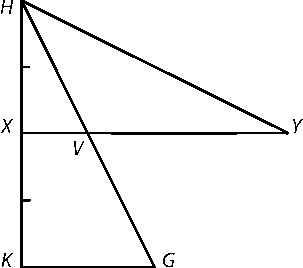
\includegraphics[width=0.38\textwidth]{gesamttex/edit_VIII,3/images/LH_35_09_15_012-013_d2.pdf}}%\\
 \vspace{0.5em}%
 \centerline{\lbrack\textit{Fig.~2}\rbrack}%
 \label{LH_35_09_15_012r_Fig.2}%
 \vspace{1.0em}%
%
%
\pstart%
%
%  !!!!! Getrixt: Folgende Cfootnote hängt eigentlich an das Diagramm Fig. 2. !!!!!
\edtext{}{%
\lemma{\hspace*{1,6mm}\lbrack\textit{Fig.~2}\rbrack}\killnumber%
\Cfootnote{Ein in \textit{L} befindlicher, gestrichener Erstentwurf des Diagramms wird hier \mbox{nicht} wiedergegeben.}}%
%
His\edlabel{LH_35_09_15_012r_utsubduplrt_utrc}
jam positis\lbrack,\rbrack\
circa duos ejusdem chordae diversis gradibus tensae
\edtext{status%
\protect\index{Sachverzeichnis}{chorda tensa}%
\protect\index{Sachverzeichnis}{gradus tensionis}%
\protect\index{Sachverzeichnis}{status chordae}
et}{\lemma{status~\textbar~,}\Bfootnote{\textit{streicht Hrsg.}~%
\textbar\ et%
~\textit{L}}}
%
in singulis vibrationes\protect\index{Sachverzeichnis}{vibratio chordae} ita
\edtext{ratiocinabimur.
\edlabel{LH_35_09_15_012r_dskjghrui-1}Sit}{%
\lemma{ratiocinabimur.}\Bfootnote{%
\textit{(1)}~Sint
\textit{(2)}~Sit%
~\textit{L}}}
\edtext{}{%
{\xxref{LH_35_09_15_012r_dskjghrui-1}{LH_35_09_15_012r_dskjghrui-2}}%
{\lemma{Sit \lbrack...\rbrack\ $PLM$}\Cfootnote{%
Siehe das Diagramm \lbrack\textit{Fig.~1}\rbrack\ in N.~8\textsubscript{3}, S.~\pageref{LH_35_09_15_010r_fig.1}.}}}%
chorda tensa $BAQ,$\protect\index{Sachverzeichnis}{chorda tensa}
eadem tendatur ulterius in $PLM.$\edlabel{LH_35_09_15_012r_dskjghrui-2}
Longitudo\protect\index{Sachverzeichnis}{longitudo chordae}
prius erat $BA,$ nunc est $ML.$
Unde
\edtext{erit: $BA$ : $LM$}{%
\lemma{erit:}\Bfootnote{%
\textit{(1)}~$AQ : LP$
\textit{(2)}~$BA : LM$%
~\textit{L}}}%
$\displaystyle\ \squaredots\ LP$ quadr. :
\edtext{$AQ$ quadr.
In ipsa $ML$ sumatur}{%
\lemma{$AQ$}\Bfootnote{%
\hspace{-0,5mm}quadr.
\textit{(1)}~Sumatur
\textit{(2)}~In ipsa $ML$
\textit{(3)}~In ipsa $ML$ sumatur%
~\textit{L}}}
%
$LR$ aequ. $BA$
et in chorda $BAQ$ assumatur cylinder $BAS$\protect\index{Sachverzeichnis}{cylinder}
per omnia aequalis et similis chordae $RLP.$
\edtext{Habemus duas chordas $BAS$ et $RLP$}{%
\lemma{Habemus}\Bfootnote{%
\hspace{-0,5mm}duas chordas $BAS$ et $RLP$ \textit{gestr.~u. wieder gültig gemacht~L}}}
sola tensione differentes.\protect\index{Sachverzeichnis}{tensio chordae}
Tempus quo\protect\index{Sachverzeichnis}{tempus restitutionis}
\edtext{chorda $BAS$ per se pulsata\protect\index{Sachverzeichnis}{chorda pulsata}}{%
\lemma{chorda}\Bfootnote{%
\textit{(1)}~$AB$
\textit{(2)}~$BAS$
\textit{(a)}~per se
\textit{(b)}~pulsa
\textit{(c)}~per se pulsata%
~\textit{L}}}
restituitur\lbrack,\rbrack\
sit $s,$ et
\edtext{tempus\protect\index{Sachverzeichnis}{tempus restitutionis}
quo altera $RLP$ restitueretur
per se pulsata\protect\index{Sachverzeichnis}{chorda pulsata}}{%
\lemma{tempus}\Bfootnote{%
\textit{(1)}~quo altera $RLP$
\textit{(a)}~restitueretur
\textit{(b)}~per se pulsata restitutitur seu
\textit{(aa)}~qua
\textit{(bb)}~vibratur
\textit{(2)}~quo altera \lbrack...\rbrack\ se pulsata%
~\textit{L}}}\lbrack,\rbrack\
sit $p.$
Ratiocinatio\protect\index{Sachverzeichnis}{ratiocinatio}
igitur talis prodibit;
modo notetur me
% \edtext{}{%
% \lemma{notetur}\Bfootnote{%
% \textit{(1)}~me
% \textit{(2)}~me%
% ~\textit{L}}}
hic tempus vibrandi\protect\index{Sachverzeichnis}{tempus vibrandi}
vocare vibrationem.\protect\index{Sachverzeichnis}{vibratio chordae}
%
\lbrack12~v\textsuperscript{o}\rbrack\ % Blatt 12v
%
Vibratio $BAS$ \!:\! vibratio $RLP$ $\squaredots\,$ $s$ \!:\! $p$
\edtext{ex hypothesi.\protect\index{Sachverzeichnis}{hypothesis}}{%
\lemma{ex}\Bfootnote{%
\hspace{-0,5mm}hypothesi
\textit{erg.~L}}}
Jam vibratio $BAS$ aequ. vibr. $BAQ,$
quia
\edtext{\edlabel{LH_35_09_15_012v_crassitiessuperflua-1}crassities non variat tempus vibrandi;\edlabel{LH_35_09_15_012v_crassitiessuperflua-2}\protect\index{Sachverzeichnis}{tempus vibrandi}}{%
\lemma{crassities \lbrack...\rbrack\ vibrandi}\Cfootnote{%
% Siehe N.~??A10\textsubscript{2}, S.~\refpassage{LH_35_09_15_009v_crassitiessuperflua-1}{LH_35_09_15_009v_crassitiessuperflua-2}.
Siehe \cite{00044}H.~\textsc{Fabri}, \textit{Physica}, tract.~III, lib.~II, prop.~223; 224 (Bd.~II, Lyon 1670, S.~215b; 216a; 216b).}}
%
\edtext{ergo vibr. $BAQ$}{%
\lemma{ergo}\Bfootnote{%
\textit{(1)}~$BAQ$
\textit{(2)}~vibr. $BAQ$%
~\textit{L}}}
: vibr. $RLP$ $\squaredots\,$ $s$ : $p.$
\pend%
%
\pstart%
Porro\protect\index{Sachverzeichnis}{vibratio chordae}
vibr. \!$RLP$ \!: vibr. \!$MLP$ $\squaredots\,$ $RL$ \!:\! $ML,$
quia tempora\protect\index{Sachverzeichnis}{tempus vibrationis}
quibus vibrantur vel restituuntur duae chordae similes
aeque tensae\protect\index{Sachverzeichnis}{chorda tensa}
sola longitudine differentes
sunt ut longitudines\protect\index{Sachverzeichnis}{longitudo chordae}\lbrack,\rbrack\
nempe brevior breviori tempore restituitur\protect\index{Sachverzeichnis}{tempus restitutionis}
in ea ratione in qua brevior est,
de quo
\edtext{supra.}{%
\lemma{supra}\Cfootnote{%
N.~8\textsubscript{2}, S.~\refpassage{LH_35_09_15_009v_utlong-1}{LH_35_09_15_009v_utlong-2};
N.~8\textsubscript{1}, S.~\refpassage{LH_35_09_15_007v_vrws2-1}{LH_35_09_15_007v_vrws2-2}.}}%
\pend%
%
\pstart%
Ergo
\edtext{componendo erit vibr.\protect\index{Sachverzeichnis}{vibratio chordae}}{%
\lemma{componendo}\Bfootnote{%
\textit{(1)}~vibr.
\textit{(2)}~erit vibr.%
~\textit{L}}}%
$\,BAQ : \text{vibr.}\, MLP\, \squaredots\ s : p. \smallfrown (RL : ML\ \text{vel})\ AB : ML.$
Igitur%
\protect\index{Sachverzeichnis}{chorda tensa}%
\textso{ chordae }%
\edtext{\textso{alicuius}}{%
\lemma{\textso{alicuius}}\Bfootnote{\textit{erg.~L}}}%
\textso{ diversimode tensae vibrationes }%
\protect\index{Sachverzeichnis}{vibratio chordae}%
\edtext{\textso{seu vibrandi tempora}}{%
\lemma{\textso{seu}}\Bfootnote{%
\hspace{-1,1mm}\textso{ vibrandi tempora} \textit{erg.~L}}}%
\protect\index{Sachverzeichnis}{tempus vibrandi}%
\textso{ sunt inter se in composita ratione ex ratione tensionum seu ponderum seu longitudinum }%
\protect\index{Sachverzeichnis}{tensio chordae}%
\protect\index{Sachverzeichnis}{pondus tendens}%
\protect\index{Sachverzeichnis}{longitudo chordae}%
(\phantom)\hspace*{-1.2mm}%
haec enim
\edtext{coincidunt hoc casu
ut
\edtext{supra}{%
\lemma{supra}\Cfootnote{%
N.~8\textsubscript{2}, S. \refpassage{LH_37_09_15_012v_udzfgouzdfg-1}{LH_37_09_15_012v_udzfgouzdfg-2}.}}
ostensum est}{%
\lemma{coincidunt}\Bfootnote{%
\textit{(1)}~ut supra
\textit{(2)}~hoc casu ut supra ostensum 
\textit{(a)}~est
\textit{(b)}~est%
~\textit{L}}}%
\phantom(\hspace*{-1.2mm})%
\textso{ et ratione temporum quibus duae aliae }%
\edtext{\textso{chordae his tensionibus praeditae, iisque solis}}{%
\lemma{\textso{chordae}}\Bfootnote{%
\textit{(1)}~iisd
\textit{(2)}~sola te
\textit{(3)}~iis
\textit{(4)}~\textso{his tensionibus praeditae, iisque solis}%
~\textit{L}}}%
\textso{ differentes, vibrarentur.}%
\protect\index{Sachverzeichnis}{tempus vibrationis}%
\protect\index{Sachverzeichnis}{tensio chordae}%
\protect\index{Sachverzeichnis}{vibratio chordae}
\edtext{Quod etiam eodem modo
\edtext{supra}{%
\lemma{supra}\Cfootnote{%
N.~8\textsubscript{3}, S.~\refpassage{LH_35_09_15_010v_rtcmpst-1}{LH_35_09_15_010v_rtcmpst-2}.}}
jam probaveramus,
et nunc repetere visum est.}{%
\lemma{Quod}\Bfootnote{%
\hspace{-0,5mm}etiam \lbrack...\rbrack\ supra jam
\textit{(1)}~potueramus et ja
\textit{(2)}~probaveramus, et \lbrack...\rbrack\ visum est.
\textit{erg.~L}}}
\pend%
%
\pstart%
Si\edlabel{LH_35_09_15_012v_nonuttensio-1}
\edtext{ergo harum}{%
\lemma{ergo}\Bfootnote{%
\hspace{-0,5mm}\textbar~ut supra pagina praecedente tentavimus \textit{gestr.}~%
\textbar\ harum%
~\textit{L}}}
chordarum vibrationes\protect\index{Sachverzeichnis}{vibratio chordae}
essent reciproce ut tensiones,\protect\index{Sachverzeichnis}{tensio chordae}
seu si $s$ \!:\! $p$
\!$\squaredots$\!
$ML$ \!:\! $AB,$
fiet vibr. \!$BAQ$ \!:\! vibr. \!$MLP$ \!$\squaredots$\! $ML$ \!:\! $AB.$ \!$\smallfrown$\! $AB$ \!:\! $ML.$
Ergo fiet vibr. \!$BAQ$ aequ. \mbox{vibr.} \!$MLP.$
Quod est
\edtext{absurdum,
eadem enim chorda magis tensa\protect\index{Sachverzeichnis}{chorda tensa}
utique vibrationes\protect\index{Sachverzeichnis}{vibratio chordae} habet celeriores.
Itaque}{%
\lemma{absurdum,}\Bfootnote{%
\textit{(1)}~itaque
\textit{(2)}~eadem enim \lbrack...\rbrack\ celeriores. Itaque
\textit{L}}}%
\textso{ absurdum est, duarum chordarum sola tensione differentium tempora vibrandi esse ut tensiones }%
\protect\index{Sachverzeichnis}{tempus vibrandi}\protect\index{Sachverzeichnis}{tensio chordae}%
\edtext{\textso{reciproce.}%
\edlabel{LH_35_09_15_012v_nonuttensio-2}
\newline%
%
\indent%
% ANFANG DER MARGINALIE
\edtext{}{%
{\xxref{LH_35_09_15_012v_marg-1}{LH_35_09_15_012v_marg-2}%
}{\lemma{\textit{Am Rand:}}\Afootnote{%
$\displaystyle\sqrt{\protect\vphantom{\protect\mathstrut\frac{ML}{AB}}}\!\frac{ML}{AB}$%
\textsuperscript{[a]}
aequ.
$\displaystyle\frac{s}{p}\smallfrown\frac{AB}{ML}.$
Ergo
$\displaystyle\frac{s}{p}$
aequ.
$\displaystyle\sqrt{\protect\vphantom{\protect\mathstrut\frac{ML^3}{AB^3}}}\!\frac{ML^3}{AB^3}.$
\\%
\\%
\\%
\footnotesize{%
\textsuperscript{[a]}
\textit{(1)}~$\displaystyle\sqrt{\protect\vphantom{\protect\mathstrut\frac{AB}{ML}}}\!\frac{AB}{ML}\, \smallfrown$ 
\textit{(2)}~$\displaystyle\sqrt{\protect\vphantom{\protect\mathstrut\frac{ML}{AB}}}\!\frac{ML}{AB}$
}}}}% \ %
Hinc%
\edlabel{LH_35_09_15_012v_marg-1}\edlabel{LH_35_09_15_013r_widerlegung-1}
patet%
\protect\index{Sachverzeichnis}{tensio chordae}%
\protect\index{Sachverzeichnis}{tempus vibrandi}%
\textso{ si duarum chordarum sola tensione differentium tempora vibrandi
essent in subduplicata ratione reciproca tensionum }}{%
\lemma{\textso{reciproce.}}\Bfootnote{%
\textit{(1)}~Si essent
\textit{(2)}~Hinc patet \textso{si}
\textit{(a)}~\textso{essent}
\textit{(b)}~\textso{duarum chordarum} \lbrack...\rbrack\ \textso{vibrandi essent}
\textit{(aa)}~,~ut
\textit{(bb)}~\textso{in subduplicata ratione reciproca tensionum}%
~\textit{L}}}%
\edtext{seu si sint pondera\protect\index{Sachverzeichnis}{pondus tendens}
vel tensiones\protect\index{Sachverzeichnis}{tensio chordae}
in duplicata ratione reciproca vibrationum\protect\index{Sachverzeichnis}{vibratio chordae}
ut \edtext{paulo ante}{\lemma{paulo ante}\Cfootnote{%
S.~\refpassage{LH_35_09_15_012r_utsubduplrt-1}{LH_35_09_15_012r_utsubduplrt-2}.% \hspace*{10mm}
}}
\edtext{ex hypothesi fictitia\protect\index{Sachverzeichnis}{hypothesis fictitia}}{%
\lemma{ex hypothesi fictitia}\Cfootnote{%
Siehe S.~\refpassage{LH_35_09_15_012r_utsubduplrt-3}{LH_35_09_15_012r_utsubduplrt-4}.}}
incrementi uniformis\protect\index{Sachverzeichnis}{incrementum motus uniforme} tentavimus}{%
\lemma{seu}\Bfootnote{%
\hspace{-0,5mm}si \lbrack...\rbrack\ ratione reciproca
\textit{(1)}~tensionum
\textit{(2)}~vibrationum ut
\textit{(a)}~pagi
\textit{(b)}~paulo ante \lbrack...\rbrack\ uniformis tentavimus
\textit{erg.~L}}}
(\phantom)\hspace*{-1.2mm}%
seu si $s$\,:\,$p$\,%
$\squaredots$\,%
$\displaystyle\sqrt{\protect\vphantom{\protect\mathstrut ML}}\!ML$\,:\,%
$\displaystyle\sqrt{\protect\vphantom{\protect\mathstrut AB}}\!AB$%
\phantom(\hspace*{-1.2mm})\textso{ }%
\edtext{\textso{tunc }%
ut \edtext{pagina praecedenti\protect\index{Sachverzeichnis}{pagina praecedens}}{%
\lemma{pagina praecedenti}\Cfootnote{%
Siehe S.~\refpassage{LH_35_09_15_012r_utsubduplrt-1}{LH_35_09_15_012r_utsubduplrt-2}.}} % LH_35_09_15_012r_utsubduplrt-1 LH_35_09_15_012r_utsubduplrt-2 
tentavimus,%
\protect\index{Sachverzeichnis}{chorda tensa}%
\protect\index{Sachverzeichnis}{tempus vibrandi}%
\textso{ ejusdem chordae diversimode tensae tempora vibrandi fore in subduplicata}}{%
\lemma{\textso{tunc}}\Bfootnote{%
\textit{(1)}~\textso{fore}
\textit{(2)}~\textbar~ut pagina praecedenti tentavimus, \textit{erg.}~%
\textbar\ \textso{ejusdem chordae} \lbrack...\rbrack\ \textso{fore in}
\textit{(a)}~\textso{dupli}
\textit{(b)}~\textso{subduplicata}%
~\textit{L}}}%
\textso{ ratione % }%
% \edtext{\lbrack reciproca\rbrack}{\lemma{reciproca}\Bfootnote{\textit{erg. Hrsg.}}}%
% \textso{
tensionum.}\protect\index{Sachverzeichnis}{tensio chordae}%
\edlabel{LH_35_09_15_012v_marg-2}
% ENDE DER MARGINALIE 
% \newline%
%
% \indent%
Nam
\edtext{si in ratione composita $s$ \!:\! $p.$ \!$\smallfrown$\! $AB$ \!:\! $ML$ pro}{%
\lemma{si}\Bfootnote{%
\textit{(1)}~pro
\textit{(2)}~in ratione composita $s$ \!:\! $p.$ \!$\smallfrown$\! $AB$ \!:\! $ML$
\textit{(a)}~pro
\textit{(b)}~pro%
~\textit{L}}}
$s$ \!:\! $p$ substituas
$\displaystyle\sqrt{\protect\vphantom{\protect\mathstrut ML}}\!ML$ \!:\!
$\displaystyle\sqrt{\protect\vphantom{\protect\mathstrut AB}}\!AB,$
fiet
$\displaystyle\sqrt{\protect\vphantom{\protect\mathstrut ML}}\!ML$ \!:\!
$\displaystyle\sqrt{\protect\vphantom{\protect\mathstrut AB}}\!AB.$ \!$\smallfrown$\!
$AB$ \!:\! $ML,$
quod est
\!$\squaredots$\!
$\displaystyle\sqrt{\protect\vphantom{\protect\mathstrut AB}}\!AB$ \!:\!
$\displaystyle\sqrt{\protect\vphantom{\protect\mathstrut ML}}\!ML.$
Ergo vibr. $BAQ$ \!:\! vibr. $MLP$
\!$\squaredots$\!
$\displaystyle\sqrt{\protect\vphantom{\protect\mathstrut AB}}\!AB$ \!:\!
$\displaystyle\sqrt{\protect\vphantom{\protect\mathstrut ML}}\!ML.$
Seu si
\edtext{chorda $BAQ$ tensa\protect\index{Sachverzeichnis}{chorda tensa} pondere $E,$
alio pondere quadruplo\protect\index{Sachverzeichnis}{pondus tendens quadruplum} $N$ extendatur
in quadruplae longitudinis\protect\index{Sachverzeichnis}{longitudo chordae} chordam $MLP,$
ita ut $LM$ sit quadrupla $AB,$}{%
\lemma{chorda}\Bfootnote{%
\textit{(1)}~$LM$ sit quad
\textit{(2)}~$BAQ$ tensa \lbrack...\rbrack\ sit quadrupla $AB,$%
~\textit{L}}}
erit
$\displaystyle\sqrt{\protect\vphantom{\protect\mathstrut AB}}\!AB$ \!:\!
$\displaystyle\sqrt{\protect\vphantom{\protect\mathstrut ML}}\!ML$
\!$\squaredots$\! 1 \!:\! 2,
adeoque chorda $AB$ minus tensa
\edtext{tempore minori ut 1 absolveret}{%
\lemma{tempore}\Bfootnote{%
\textit{(1)}~dimidio absolveret
\textit{(2)}~minori ut 1 absolveret%
~\textit{L}}}
vibrationem,
quam magis tensa\protect\index{Sachverzeichnis}{chorda tensa}
quae tempore ut 2.\protect\index{Sachverzeichnis}{tempus vibrationis}
%
\lbrack13~r\textsuperscript{o}\rbrack\ % Blatt 13r
%
Quod est absurdum,
itaque%
\textso{ absurdum est duarum chordarum sola tensione differentium }%
\protect\index{Sachverzeichnis}{chorda tensa}%
tempora vibrandi\protect\index{Sachverzeichnis}{tempus vibrandi}
esse in ratione subduplicata reciproca tensionum.\protect\index{Sachverzeichnis}{tensio chordae}
\edtext{Quod mirum non est,
quia id tentaminis\protect\index{Sachverzeichnis}{tentamen} solum causa
\edtext{secunda retro pagina}{%
\lemma{secunda \lbrack...\rbrack\ pagina}\Cfootnote{%
S.~\refpassage{LH_35_09_15_012r_utsubduplrt-1}{LH_35_09_15_012r_utsubduplrt-2}.}}
\edtext{ex falsa hypothesi\protect\index{Sachverzeichnis}{hypothesis falsa}}{%
\lemma{ex falsa hypothesi}\Cfootnote{%
Siehe S.~\refpassage{LH_35_09_15_012r_utsubduplrt-3}{LH_35_09_15_012r_utsubduplrt-4}.}}
aequalis accelerationis\protect\index{Sachverzeichnis}{acceleratio aequalis} duximus.%
\edlabel{LH_35_09_15_013r_widerlegung-2}
% Unde patet quam male ratiocinati sint
% \edtext{Beaunius%
% \protect\index{Namensregister}{\textso{Beaune} (Beaunius), Florimond de 1601\textendash1652}
% apud Mersennum%
% \protect\index{Namensregister}{\textso{Mersenne} (Mersennus), Marin 1588\textendash1648}
% in \textit{Phaenomenis Ballisticis}
% prop.~37}{%
% \lemma{Beaunius \lbrack...\rbrack\ prop.~37}\Cfootnote{%
% \cite{01227}M.~\textsc{Mersenne}, \textit{Ballistica% et acontismologia
% }, prop.~36, Paris 1644, S.~132.
% Der Verweis auf prop.~37 ist irrtümlich.}}
% et cum Beaunio%
% \protect\index{Namensregister}{\textso{Beaune} (Beaunius), Florimond de 1601\textendash1652}
% Cartesius%
% \protect\index{Namensregister}{\textso{Descartes} (Cartesius, des Cartes), Ren\'{e} 1596\textendash1650}
% in Epistola 84 Tomi III.\protect\index{Sachverzeichnis}{epistola}
% \edtext{Supponit enim Cartesius%
% \protect\index{Namensregister}{\textso{Descartes} (Cartesius, des Cartes), Ren\'{e} 1596\textendash1650}
% nullum errorem notabilem\protect\index{Sachverzeichnis}{error notabilis} proditurum
% si incrementa\protect\index{Sachverzeichnis}{incrementum velocitatis} ponantur semper proposita.}{%
% \lemma{Supponit \lbrack...\rbrack\ proposita}\Cfootnote{%
% \cite{01226}R.~\textsc{Descartes}, Brief an M.~Mersenne vom 30. April 1639
% (\cite{00209}\textit{DL}~III, Nr.~84, S.~483f.; \cite{00120}\textit{DO}~II, Nr.~160, S.~534\textendash536).}}
% Neque responsum est ab iis ad quaestionem\protect\index{Sachverzeichnis}{quaestio}
% a Mersenno propositam, sed ad aliam.
% \edtext{Quaerebat enim Mersennus%
% \protect\index{Namensregister}{\textso{Mersenne} (Mersennus), Marin 1588\textendash1648}
% cur eadem chorda\protect\index{Sachverzeichnis}{chorda tensa}
% quadruplo pondere\protect\index{Sachverzeichnis}{pondus tendens quadruplum}
% ad octavam\protect\index{Sachverzeichnis}{octava} usque tendenda sit.}{%
% \lemma{Quaerebat \lbrack...\rbrack\ sit}\Cfootnote{%
% Vgl. \cite{01227}\textsc{Mersenne}, \textit{Ballistica}, prop.~36, S.~128.%
% prop.~36 lautet:
% \textit{Causam investigare ob quam vires nervum tendentes sint in ratione velocitatum, quibus movetur, duplicata.}
% Vgl. \cite{01227}\textsc{Mersenne}, \textit{Ballistica}, S.~128.
% }}
% Aliud autem est eandem chordam ad octavam perduci,
% aliud est duas diversas chordas
% sola tensione\protect\index{Sachverzeichnis}{tensio chordae} differentes,
% octava\protect\index{Sachverzeichnis}{octava} distare\lbrack,\rbrack\
% quia eadem chorda diversimode tensa\protect\index{Sachverzeichnis}{chorda tensa}
% a se ipsa non tantum \lbrack\textit{Text bricht ab.}\rbrack%
}{%
\lemma{Quod}\Bfootnote{
\hspace{-0,5mm}mirum \lbrack...\rbrack\ solum causa
\textit{(1)}~penultim
\textit{(2)}~secunda retro \lbrack...\rbrack\ accelerationis duximus.
% \textit{(a)}~A
% \textit{(b)}~Unde
% \textit{(aa)}~quam
% \textit{(bb)}~patet quam \lbrack...\rbrack\ apud Mersennum
% \textit{(aaa)}~in C
% \textit{(bbb)}~in Phaenomenis \lbrack...\rbrack\ Beaunio Cartesius
% \textit{(aaaa)}~prop.
% \textit{(bbbb)}~in
% \textit{(aaaaa)}~Epistolis Tomi III lettre
% \textit{(bbbbb)}~Epistola 84 \lbrack...\rbrack\ nullum errorem
% \textit{(aaaaa-a)}~deprehendi si po
% \textit{(bbbbb-b)}~notabilem proditurum \lbrack...\rbrack\ differentes, octava
% \textit{(aaaaa-aa)}~differre
% \textit{(bbbbb-bb)}~distare quia \lbrack...\rbrack\ non tantum
\textit{erg.~L}}}%
%    %    %    %    %
\edtext{}{\lemma{\textit{Am Rand,}}\Afootnote{%
\hspace{-0,5mm}\textit{durch ein gestr. Einfügungszeichen eingeleitet:}
\protect\rule[-0.8mm]{0mm}{0mm}Unde%
\textsuperscript{[a]} %%%%
patet quam male ratiocinati \protect\rule[-0.8mm]{0mm}{0mm}sint
Beaunius\protect\index{Namensregister}{\textso{Beaune} (Beaunius), Florimond de 1601\textendash1652}%
\textsuperscript{[b]} %%%%
apud Mersennum\protect\index{Namensregister}{\textso{Mersenne} (Mersennus), Marin 1588\textendash1648}%
\textsuperscript{[c]} %%%%
in \textit{Phaenomenis Ballisticis} prop.~37
et cum Beaunio\protect\index{Namensregister}{\textso{Beaune} (Beaunius), Florimond de 1601\textendash1652}
\protect\rule[-0.8mm]{0mm}{0mm}Cartesius\protect\index{Namensregister}{\textso{Descartes} (Cartesius, des Cartes), Ren\'{e} 1596\textendash1650}%
\textsuperscript{[d]} %%%%
in Epistola 84 Tomi III.\protect\index{Sachverzeichnis}{epistola}
Supponit%
\textsuperscript{[e]} %%%%
enim Cartesius\protect\index{Namensregister}{\textso{Descartes} (Cartesius, des Cartes), Ren\'{e} 1596\textendash1650}
nullum errorem%
\textsuperscript{[f]} %%%%
\protect\rule[-0.8mm]{0mm}{0mm}notabilem\protect\index{Sachverzeichnis}{error notabilis} proditurum
si incrementa\protect\index{Sachverzeichnis}{incrementum velocitatis} ponantur semper proposita.
Neque responsum \protect\rule[-1.7mm]{0mm}{0mm}est ab iis ad quaestionem\protect\index{Sachverzeichnis}{quaestio}
a Mersenno propositam, sed ad aliam.
Quaerebat%
\textsuperscript{[g]} %%%%
enim \protect\rule[-1.8mm]{0mm}{0mm}Mersennus\protect\index{Namensregister}{\textso{Mersenne} (Mersennus), Marin 1588\textendash1648}
cur eadem chorda\protect\index{Sachverzeichnis}{chorda tensa}
quadruplo pondere\protect\index{Sachverzeichnis}{pondus tendens quadruplum}
ad octavam\protect\index{Sachverzeichnis}{octava} usque tendenda sit.
%
Aliud \protect\rule[-0.8mm]{0mm}{0mm}autem est eandem chordam ad octavam perduci,
aliud est duas diversas chordas
sola tensione\protect\index{Sachverzeichnis}{tensio chordae} \protect\rule[-1.2mm]{0mm}{0mm}differentes,
octava\protect\index{Sachverzeichnis}{octava}%
\textsuperscript{[h]} %%%%
distare\lbrack,\rbrack\
quia eadem chorda diversimode tensa\protect\index{Sachverzeichnis}{chorda tensa}
a se ipsa non tantum \lbrack\textit{Text bricht ab.}\rbrack%
\\%
\\%
% \\%
\footnotesize{%
%%%%
\textsuperscript{[a]}~%
Unde
\textit{(1)}~quam
\textit{(2)}~patet quam%
~\textit{L}
\quad
%%%%
\textsuperscript{[b]}~%
Beaunius \lbrack...\rbrack\ prop.~37: \cite{01227}M.~\textsc{Mersenne}, \textit{Ballistica}, prop.~36 (Paris 1644, S.~132). Der Verweis auf prop.~37 ist irrtümlich.
\quad
%%%%
\textsuperscript{[c]}~%
Mersennum
\textit{(1)}~in C
\textit{(2)}~in Phaenomenis Ballisticis%
~\textit{L}
\quad
%%%%
\textsuperscript{[d]}~%
Cartesius
\textit{(1)}~prop.
\textit{(2)}~in
\textit{(a)}~Epistolis Tomi III lettre
\textit{(b)}~Epistola 84 Tomi III.%
~\textit{L}
\quad
%%%%
\textsuperscript{[e]}~%
Supponit \lbrack...\rbrack\ proposita: \cite{01226}R.~\textsc{Descartes}, Brief an M.~Mersenne vom 30. April 1639 (\cite{00209}\textit{DL}~III, Nr.~84, S.~483f.; \cite{00120}\textit{DO}~II, Nr.~160, S.~534\textendash536).
\quad
%%%%
\textsuperscript{[f]}~%
errorem
\textit{(1)}~deprehendi si po
\textit{(2)}~notabilem proditurum si incrementa ponantur%
~\textit{L}
\quad
%%%%
\textsuperscript{[g]}~%
Quaerebat \lbrack...\rbrack\ tendenda sit: Vgl. \cite{01227}\textsc{Mersenne}, \textit{Ballistica}, prop.~36 (S.~128).
\quad
%%%%
\textsuperscript{[h]}~%
octava
\textit{(1)}~differre
\textit{(2)}~distare%
~\textit{L}
%%%%
}
}}
\pend%
\newpage
%
\pstart%
Si verum est
\edtext{quod ajunt}{%
\lemma{quod ajunt}\Cfootnote{%
Es ist nicht ersichtlich, auf wen Leibniz hier anspielt.
% ??? Mersenne? Galilei? Fabri?
}}
experientia\protect\index{Sachverzeichnis}{experientia}
\edtext{comprobari;%
\textso{ chordae diversimode tensae}%
\protect\index{Sachverzeichnis}{chorda diversimode tensa}%
\textso{ tempora vibrandi}%
\protect\index{Sachverzeichnis}{tempus vibrandi}%
\textso{ esse in ratione reciproca duplicata tensionum}%
\protect\index{Sachverzeichnis}{tensio chordae}%
\textso{ }%
seu%
\textso{ longitudinum}\protect\index{Sachverzeichnis}{longitudo chordae}%
\textso{ seu ponderum,}\protect\index{Sachverzeichnis}{pondus tendens}
idque%
\textso{ }%
\edtext{\textso{circiter,}}{%
\lemma{\textso{circiter}}\Cfootnote{%
Doppelt unterstrichen.}}%
\textso{ }%
seu chordam $BAQ$}{%
\lemma{comprobari;}\Bfootnote{%
\textit{(1)}~duarum chor
\textit{(2)}~tensionum ejusdem
\textit{(3)}~\textso{chordae diversimode tensae}
\textit{(a)}~vibrationes
\textit{(b)}~\textso{tempora vibrandi} \lbrack...\rbrack\ \textso{duplicata tensionum}
\textit{(aa)}~, circiter,
\textit{(bb)}~seu chordam $BA$ circiter, 
\textit{(cc)}~seu \textso{longitudinem} \lbrack...\rbrack\ seu chordam $BAQ$%
~\textit{L}}}
longitudine\protect\index{Sachverzeichnis}{longitudo chordae} subquadruplam
ejusdem chordae magis tensae\protect\index{Sachverzeichnis}{chorda tensa} $MLP$ duplo
\edtext{tempore\protect\index{Sachverzeichnis}{tempus vibrationis}
vibrationem\protect\index{Sachverzeichnis}{vibratio chordae}}{%
\lemma{tempore}\Bfootnote{%
\textit{(1)}~restitu
\textit{(2)}~vibrationem%
~\textit{L}}}
absolvere,
seu sonum edere duplo graviorem;\protect\index{Sachverzeichnis}{sonus gravis}
sequitur:%
\textso{ duarum chordarum sola tensione differentium tempora}%
\protect\index{Sachverzeichnis}{tempus vibrationis}%
\textso{ esse in ratione triplicata subduplicata reciproca tensionum,}\protect\index{Sachverzeichnis}{tensio chordae}
\!\! etiam%
\textso{ }%
\edtext{\textso{circiter,}}{%
\lemma{\textso{circiter}}\Cfootnote{%
Doppelt unterstrichen.\hspace{-2mm}}}
quod ita ostendo:
vibr.\protect\index{Sachverzeichnis}{vibratio chordae}\,$BAQ$ : vibr.\,$MLP$
$\squaredots\,$
$\displaystyle\sqrt{ML} : \sqrt{AB}$
per suppositionem experimenti\protect\index{Sachverzeichnis}{experimentum}
\edtext{supra}{%
\lemma{supra}\Cfootnote{%
S.~\refpassage{LH_35_09_15_012v_marg-1}{LH_35_09_15_012v_marg-2};
\refpassage{LH_35_09_15_012r_utsubduplrt-1}{LH_35_09_15_012r_utsubduplrt-2}.}}
dictam.\,
At vibr.\,$BAQ$ : vibr.\,$MLP$\protect\index{Sachverzeichnis}{vibratio chordae}
$\squaredots$
$s$ : $p.$ $\smallfrown$ $AB$ : $ML.$
Ergo $s$ : $p.$ $\smallfrown$ $AB$ : $ML$
$\squaredots$
$\sqrt{ML : AB}.$
Ergo $s$ : $p$
$\squaredots$
$ML$ : $AB.$ $\smallfrown$
$\sqrt{ML : AB}.$
Seu $s$ : $p$
$\squaredots$
$\sqrt{ML^3}$ :
\edtext{$\sqrt{AB^3}.$
Seu $ss$}{%
\lemma{$\sqrt{AB^3}.$}\Bfootnote{%
\hspace{-0,5mm}Seu
\textit{(1)}~$s^2$
\textit{(2)}~$ss$%
~\textit{L}}}
: $pp$ $\squaredots$ $ML^3$ : $AB^3.$
Seu\textso{ quadrata temporum quibus }%
\protect\index{Sachverzeichnis}{tempus restitutionis}%
\edtext{\textso{chordae sola tensione differentes}}{%
\lemma{\textso{chordae}}\Bfootnote{%
\textit{(1)}~\textso{tensae}
\textit{(2)}~\textso{sola tensione differentes}%
~\textit{L}}}%
\textso{ restituuntur,
erunt in ratione }%
\edtext{\textso{[reciproca]}}{%
\lemma{ \textso{reciproca}}\Bfootnote{ \textit{erg. Hrsg.}}}%
\textso{ tensionum}%
\protect\index{Sachverzeichnis}{tensio chordae}%
\textso{ }%
\edtext{(\phantom)\hspace*{-0,6mm}%
\textso{seu hoc loco ponderum sustentantium}%
\protect\index{Sachverzeichnis}{pondus sustentans}%
\phantom(\hspace*{-0,6mm})}{%
\lemma{(\phantom)\hspace*{-0,6mm}\textso{seu}\,}\Bfootnote{%
\textit{(1)}~\textso{ponderum sustentantium hoc loco}\phantom(\hspace{-0,6mm})\,
\textit{(2)}~\textso{hoc loco ponderum sustentantium}\phantom(\hspace{-0,6mm})\,%
~\textit{L}}}%
\textso{ triplicata }%
etiam%
\textso{ }%
\edtext{\textso{circiter.}}{%
\lemma{\textso{circiter}}\Cfootnote{%
Doppelt unterstrichen.}}
Sed
\edtext{quia experimentis\protect\index{Sachverzeichnis}{experimentum}}{%
\lemma{quia}\Bfootnote{%
\textit{(1)}~experimentum
\textit{(2)}~experimentis%
~\textit{L}}}
inveniri non pot\-est exacta
\edtext{proportio;\protect\index{Sachverzeichnis}{proportio exacta}
hinc}{%
\lemma{proportio;}\Bfootnote{%
\textit{(1)}~tunc
\textit{(2)}~hinc%
~\textit{L}}}
qualis ea sit
\edtext{postea%
\edtext{}{\lemma{postea}\Cfootnote{%
Siehe N.~8\textsubscript{6}.}} % \refpassage{}{}
subtiliori quam}{%
\lemma{postea}\Bfootnote{%
\textit{(1)}~accuratiori qua
\textit{(2)}~subtiliori quam%
~\textit{L}}}
in hoc
\edtext{tentamine\protect\index{Sachverzeichnis}{tentamen}
adhibere opus duximus,}{%
\lemma{tentamine}\Bfootnote{%
\textit{(1)}~adhibuimus,
\textit{(2)}~adhibere opus duximus,%
~\textit{L}}}
ratiocinandi genere erit definiendum.
\pend%
% \newpage% Rein vorläufig !!!!!
%
\pstart%
\edtext{Nunc de omnimodis restitutionibus%
\protect\index{Sachverzeichnis}{restitutio omnimoda}\protect\index{Sachverzeichnis}{restitutio chordae}
quaedam accuratius constituamus,
antequam pergamus ad vibrationes.\protect\index{Sachverzeichnis}{vibratio chordae}}{%
\lemma{Nunc}\Bfootnote{%
\hspace{-0,5mm}de omnimodis
\textit{(1)}~ratiocina
\textit{(2)}~restitutionibus quaedam \lbrack...\rbrack\ ad vibrationes.
~\textit{erg.~L}}}
\edlabel{LH_35_09_15_013r-sintheor-1}%
Nimirum a me
\edtext{inventum est}{%
\lemma{inventum est}\Cfootnote{%
Siehe N.~9, S.~\refpassage{LH_35_09_15_002v_restomn-1}{LH_35_09_15_002v_restomn-2}; \refpassage{LH_35_09_15_004r_restomn-3}{LH_35_09_15_004r_restomn-4}.}}
temporibus\protect\index{Sachverzeichnis}{tempus restitutionis}
\edtext{restitutionum}{%
\lemma{restitutionum}\Bfootnote{%
\textit{erg.~L}}}
existentibus instar angulorum\protect\index{Sachverzeichnis}{angulus}
\edtext{celeritates conceptas\protect\index{Sachverzeichnis}{celeritas concepta}}{%
\lemma{celeritates}\Bfootnote{%
\hspace{-0,5mm}conceptas
\textit{erg.~L}}}
\edtext{\lbrack seu\rbrack}{%
\lemma{seu}\Bfootnote{\textit{erg. Hrsg.}}}
spatia singulis momentis\protect\index{Sachverzeichnis}{momentum temporis}
percursa,\protect\index{Sachverzeichnis}{spatium percursum}
esse ut sinus.\protect\index{Sachverzeichnis}{sinus}%
\edlabel{LH_35_09_15_013r-sintheor-3}
Ergo describatur linea sinuum,\protect\index{Sachverzeichnis}{linea sinuum}
jam
\edtext{apud autores}{%
\lemma{apud autores}\Cfootnote{%
In einer 1673 verfassten Studie,
in der Leibniz auf fremde Untersuchungen über die trigonometrischen Kurven Bezug nimmt,
erwähnt er als Autoren,
% die sich mit der Zykloiden befasst hatten%
\textit{qui de cycloeide scripsere},
ausdrücklich: E.~Torricelli, B.~Pascal, H.~Fabri, A.~de Lalouvère und insbesondere J.~Wallis.
Siehe \textit{LSB}, VII,~4 N.~39\textsubscript{1}, S.~620.30\textendash621.2\cite{01228}.}}
celebris,
et hujus ope solvi poterit Problema\protect\index{Sachverzeichnis}{problema}
\edtext{de restitutionibus duarum chordarum\protect\index{Sachverzeichnis}{restitutio chordae}
sola tensione\protect\index{Sachverzeichnis}{tensio chordae} differentium.}{%
\lemma{de}\Bfootnote{%
\hspace{-0,5mm}restitutionibus \lbrack...\rbrack\ tensione differentium
\textit{erg.~L}}}
%
\lbrack13~v\textsuperscript{o}\rbrack\ % Blatt 13v
%
\pend%
%\newpage
\pstart%
\edtext{Centro $\beta,$}{%
\lemma{Centro $\beta$}\Cfootnote{%
Siehe \lbrack\textit{Fig.~3a}\rbrack\ auf S.~\pageref{LH_35_09_15_013v_Fig.3}.}}
%
\edtext{radio $\alpha\beta$ vel $\gamma\beta,$}{%
\lemma{radio}\Bfootnote{%
\hspace{-0,5mm}$\alpha\beta$ vel $\gamma\beta,$
\textit{erg.~L}}}
sit quadrans circuli $\alpha\beta\gamma\xi\alpha.$\protect\index{Sachverzeichnis}{quadrans circuli}
Sumatur in eo arcus\protect\index{Sachverzeichnis}{arcus circuli} $\alpha\xi$
cujus sinus $\delta\xi,$\protect\index{Sachverzeichnis}{sinus}
et
\edtext{ei aequalis $\alpha\pi$ in tangente verticis $\alpha\upsilon$}{%
\lemma{ei}\Bfootnote{%
\hspace{-0,5mm}aequalis
\textit{(1)}~et parallela $\alpha\xi,$ ita ut
\textit{(2)}~$\alpha\pi$ in tangente verticis $\alpha\upsilon$%
~\textit{L}}}
sumta\lbrack,\rbrack\
ipsi applicetur $\pi\xi\mu$ aequalis
arcui $\alpha\xi,$
idemque fiat ubique
donec ipsi maximo sinui $\alpha\upsilon$ applicetur $\upsilon\theta$
aequalis arcui
\edtext{quadrantis,\protect\index{Sachverzeichnis}{quadrans circuli}
nempe ipsi $\alpha\xi\gamma.$}{%
\lemma{quadrantis,}\Bfootnote{%
\textit{(1)}~nempe
\textit{(2)}~$\alpha\xi\gamma$
\textit{(3)}~nempe ipsi $\alpha\xi\gamma.$%
~\textit{L}}}
Erit ipsa $\alpha\mu\theta$ linea sinuum\protect\index{Sachverzeichnis}{linea sinuum}
arcubus applicatorum,
nam si ex $\mu$ demittas
\edtext{applicatam $\phi\mu$}{%
\lemma{applicatam}\Bfootnote{%
\textit{(1)}~$\mu\lambda$
\textit{(2)}~$\phi\mu$%
~\textit{L}}}
in $\alpha\beta,$
tunc posito
\edtext{abscissas $\alpha\phi$}{%
\lemma{abscissas}\Bfootnote{%
\textit{(1)}~$\alpha\beta$
\textit{(2)}~$\alpha\phi$%
~\textit{L}}}
esse arcus,\protect\index{Sachverzeichnis}{arcus circuli}
\edtext{applicatae $\phi\mu$}{%
\lemma{applicatae}\Bfootnote{%
\textit{(1)}~$\lambda\mu$
\textit{(2)}~$\phi\mu$%
~\textit{L}}}
erunt sinus.\protect\index{Sachverzeichnis}{sinus}
\edlabel{LH_35_09_15_013v-sintheor-4}%
Erunt ergo in nostro casu,
per
\edtext{alibi}{%
\lemma{alibi}\Cfootnote{%
N.~9, S.~\refpassage{LH_35_09_15_002v_restomn-1}{LH_35_09_15_002v_restomn-2}
und \refpassage{LH_35_09_15_004r_restomn-3}{LH_35_09_15_004r_restomn-4}.}}
\edtext{demonstrata,
arcus\protect\index{Sachverzeichnis}{arcus circuli} $\alpha\phi$
ut tempora\protect\index{Sachverzeichnis}{tempus restitutionis}
et sinus $\phi\mu$ ut \lbrack celeritates\rbrack\ acquisitae%
\protect\index{Sachverzeichnis}{celeritas acquisita}}{%
\lemma{demonstrata,}\Bfootnote{%
\textit{(1)}~ipsae $\alpha\lambda$ ut tempus,
\textit{(2)}~arcus
\textit{(a)}~$\alpha\lambda$
\textit{(b)}~$\alpha\phi$ ut tempora et sinus
\textit{(aa)}~$\lambda\mu$
\textit{(bb)}~$\phi\mu$ ut
\textbar~celeritas \textit{ändert Hrsg.}~%
\textbar\ acquisitae%
~\textit{L}}}
%
seu spatiorum\protect\index{Sachverzeichnis}{spatium percursum}
quae percurruntur incrementa.\protect\index{Sachverzeichnis}{incrementum spatii}%
\edlabel{LH_35_09_15_013v-sintheor-2}
Prorsus ut
\edtext{supra}{%
\lemma{supra}\Cfootnote{%
Siehe das Diagramm \lbrack\textit{Fig.~2}\rbrack\ auf S.~\pageref{LH_35_09_15_012r_Fig.2}.}}
in triangulo\protect\index{Sachverzeichnis}{triangulum} ratiocinabamur,
fingendo celeritates acquisitas\protect\index{Sachverzeichnis}{celeritas acquisita}
esse temporibus\protect\index{Sachverzeichnis}{tempus restitutionis} proportionales,
\edtext{itaque $\phi\mu$ etc. usque ad $\epsilon\theta$
existentibus ut spatiorum incrementa,\protect\index{Sachverzeichnis}{incrementum spatii}
erunt $\alpha\phi\mu\alpha$}{%
\lemma{itaque}\Bfootnote{%
\textit{(1)}~$\lambda\mu,$ $\epsilon\theta$
\textit{(2)}~$\phi\mu$ etc. usque ad $\epsilon\theta$ existentibus
\textit{(a)}~spatiorum incrementis
\textit{(b)}~ut spatiorum incrementa, erunt
\textit{(aa)}~$\alpha\lambda\mu\alpha$
\textit{(bb)}~$\alpha\phi\mu\alpha$%
~\textit{L}}}
et $\alpha\epsilon\theta\alpha$
ut ipsa spatia.\protect\index{Sachverzeichnis}{spatium percursum}
\pend%
% \newpage% Vorläufig !!!!!!!
%
\pstart%
Jam in $\alpha\beta$
\edtext{sumatur alia, $\nu\alpha$ ut}{% \lbrack linea sinuum\rbrack
\lemma{sumatur}\Bfootnote{%
\textit{(1)}~$\alpha\lambda$
\textit{(2)}~alia
\textit{(a)}~linea sinuum\protect\index{Sachverzeichnis}{linea sinuum}
\textit{(b)}~, $\nu\alpha$ ut% \textbar~linea sinuum \textit{erg. Hrsg.}~\textbar\
~\textit{L}}}
$\alpha\phi,$
et radiis $\alpha\phi,$ $\phi\psi$ describatur quadrans $\alpha\phi\psi\alpha$%
\protect\index{Sachverzeichnis}{quadrans circuli}
cujus figura sinuum sit $\alpha\lambda z\varOmega\alpha$\protect\index{Sachverzeichnis}{figura sinuum}
eritque $\alpha\lambda$ aequalis
\edtext{quadrantis}{%
\lemma{quadrantis}\Bfootnote{\textit{erg.~L}}}
arcui $\alpha\psi,$
adeoque $\alpha\lambda$ ad $\alpha\epsilon$
\edtext{(\phantom)\hspace*{-1.2mm}%
seu quadrantis\protect\index{Sachverzeichnis}{quadrans circuli} arcum}{%
\lemma{(\phantom)\hspace*{-1.2mm}seu}\Bfootnote{%
\textit{(1)}~arcum 
\textit{(2)}~quadrantis arcum%
~\textit{L}}}
$\alpha\xi\gamma$%
\phantom(\hspace*{-1.2mm})
ut radii, seu ut $\alpha\phi$
\edtext{ad $\alpha\beta,$ at}{%
\lemma{ad $\alpha\beta,$}\Bfootnote{%
\textit{(1)}~et
\textit{(2)}~at%
~\textit{L}}}
$\lambda z$ erit
(\phantom)\hspace*{-1.2mm}%
aequ. $\phi\psi$ seu%
\phantom(\hspace*{-1.2mm})
aequalis $\alpha\phi.$
Est autem figura sinuum $\alpha\lambda z\omega\alpha$
aequalis quadrato radii $\alpha\phi.$
Et figura sinuum $\alpha\epsilon\theta\mu\alpha$
aequalis quadrato radii $\alpha\beta.$
Ergo figurae sinuum sunt in
\edtext{duplicata radiorum.}{%
\lemma{duplicata}\Bfootnote{%
\textit{(1)}~quadra-
\textit{(2)}~radiorum.%
~\textit{L}}}
\pend%
%
\pstart%
Jam loco figurae sinuum\protect\index{Sachverzeichnis}{figura sinuum}
\edtext{minoris}{%
\lemma{minoris}\Bfootnote{\textit{erg.~L}}}
sumamus aliam
\edtext{figuram applicatas habentem proportionales}{%
\lemma{figuram}\Bfootnote{%
\textit{(1)}~ei pro
\textit{(2)}~applicatas habentem proportionales%
~\textit{L}}}
$\alpha\lambda\varOmega\rho\alpha,$
ita ut sit
$\displaystyle \lambda z : \lambda\varOmega \,\squaredots\, \phi\omega : \phi\rho,$
sitque figura
\edtext{sinuum minor producta}{%
\lemma{sinuum}\Bfootnote{%
\hspace{-0,5mm}minor producta
\textit{erg.~L}}}
$\alpha\lambda\varOmega\rho\alpha$
aequalis figurae sinuum majori
$\alpha\epsilon\theta\mu\alpha,$
\edtext{ideo}{%
\lemma{ideo}\Bfootnote{\textit{erg.~L}}}
debet esse $\lambda\varOmega$ ad $\lambda z$
ut figura sinu\-um major ad minorem\protect\index{Sachverzeichnis}{figura sinuum}
seu in duplicata radiorum,
\edtext{et $\lambda\varOmega$ secabit lineam sinuum\protect\index{Sachverzeichnis}{linea sinuum}
$\alpha\mu\theta$ in $\varPi$:}{%
\lemma{et}\Bfootnote{%
\hspace{-0,5mm}$\lambda\varOmega$ secabit \lbrack...\rbrack\ $\alpha\mu\theta$ in $\varPi$
\textit{erg.~L}}}
Hinc
\edtext{si $\alpha\lambda$}{%
\lemma{si}\Bfootnote{%
\textit{(1)}~$\langle\alpha\phi\rangle$
\textit{(2)}~$\alpha\lambda$%
~\textit{L}}}
sit tempus\protect\index{Sachverzeichnis}{tempus restitutionis}
quo celerior
\edtext{chorda restituitur,
et $\alpha\phi$ et $\alpha\lambda$ ut partes temporis,%
\protect\index{Sachverzeichnis}{tempus restitutionis}
erunt $\phi\rho$ et $\lambda\varOmega$}{%
\lemma{chorda}\Bfootnote{%
\textit{(1)}~restit
\textit{(2)}~vibratur
\textit{(3)}~restituitur,
\textit{(a)}~$\phi$ et
\textit{(b)}~et $\alpha\phi$
\textit{(c)}~et $\alpha\phi,$ $\alpha\lambda$ ut
\textit{(d)}~et $\alpha\phi$ et $\alpha\lambda$ ut
\textit{(aa)}~pars
\textit{(bb)}~partes temporis,
\textit{(aaa)}~erit
\textit{(bbb)}~erunt $\phi\rho$ et~%
\textit{(aaaa)}~aliae
\textit{(bbbb)}~$\lambda\omega$
\textit{(cccc)}~$\lambda\varOmega$%
~\textit{L}}}
ut celeritates acquisitae\protect\index{Sachverzeichnis}{celeritas acquisita} seu
\edtext{spatiorum decursorum\protect\index{Sachverzeichnis}{spatium decursum}
incrementa\protect\index{Sachverzeichnis}{incrementum spatii}}{%
\lemma{spatiorum}\Bfootnote{%
\textit{(1)}~incremen
\textit{(2)}~decurso
\textit{(3)}~quae
\textit{(4)}~decursorum incrementa%
~\textit{L}}}
(\phantom)\hspace*{-1.2mm}%
quia temporibus\protect\index{Sachverzeichnis}{tempus restitutionis} existentibus ut
\edtext{arcus\protect\index{Sachverzeichnis}{arcus circuli}
$\alpha\phi$
(\phantom)\hspace*{-1.2mm}%
vel $\alpha\nu$%
\phantom(\hspace*{-1.2mm}),
$\alpha\lambda$
(\phantom)\hspace*{-1.2mm}%
vel $\alpha\psi$%
\phantom(\hspace*{-1.2mm}),}{%
\lemma{arcus}\Bfootnote{%
\textit{(1)}~$\alpha\phi,$ $\alpha\lambda$
\textit{(2)}~$\alpha\phi$
(\phantom)\hspace*{-1.2mm}%
vel $\alpha\nu$%
\phantom(\hspace*{-1.2mm}),
$\alpha\lambda$
(\phantom)\hspace*{-1.2mm}%
vel $\alpha\psi$%
\phantom(\hspace*{-1.2mm}),%
~\textit{L}}}
% \edtext{\lbrack celeritates acquisitae seu spatiorum incrementa\rbrack}{%
% \lemma{celeritates}\Bfootnote{%
% \hspace*{-0,5mm}acquisitae seu spatiorum incrementa
% \textit{erg. Hrsg.}}}
\edtext{sunt ut sinus\protect\index{Sachverzeichnis}{sinus}
$\phi\omega,$ $\lambda z$%
\phantom(\hspace*{-1.2mm}).}{%
\lemma{sunt \lbrack...\rbrack\ $\phi\omega,$ $\lambda z$}\Cfootnote{%
Als Subjekt sind \textit{celeritates acquisitae seu spatiorum incrementa} zu verstehen.}}
%
Ergo tota area figurae $\alpha\lambda\varOmega\rho\alpha$%
\protect\index{Sachverzeichnis}{figura sinuum}
erit ut
\edtext{spatium, et ut}{%
\lemma{spatium,}\Bfootnote{%
\textit{(1)}~utque
\textit{(2)}~et ut%
~\textit{L}}}
spatia\protect\index{Sachverzeichnis}{spatium decursum}
quae inaequalibus temporibus\protect\index{Sachverzeichnis}{tempus restitutionis}
decurruntur a chordis\protect\index{Sachverzeichnis}{chorda tensa}
aequalia
\edtext{sunt}{%
\lemma{sunt}\Bfootnote{\textit{erg.~L}}}%
\lbrack,\rbrack\
ita et $\alpha\lambda\varOmega\rho\alpha$
\edtext{erit}{%
\lemma{erit}\Bfootnote{\textit{erg.~L}}}
aequ.
\edtext{$\alpha\epsilon\theta\mu\alpha.$}{%
\lemma{$\alpha\epsilon\theta\mu\alpha.$}\Bfootnote{%
\hspace{-0,5mm}\textbar~Ipsae autem $\lambda\mu,$ $\lambda\omega$ inter se erunt
ut impetus\protect\index{Sachverzeichnis}{impetus restitutionis}
seu tensiones\protect\index{Sachverzeichnis}{tensio chordae} \textit{gestr.}~\textbar%
~\textit{L}}}%
\edtext{}{%
\lemma{\hspace*{1,6mm}\lbrack\textit{Fig.~3a}\rbrack\ auf S.~\pageref{LH_35_09_15_013v_Fig.3}}\killnumber\Cfootnote{%
Die Wiedergabe des Diagramms folgt möglichst getreu der Beschreibung in N.~8\textsubscript{4} und 8\textsubscript{5}.
Die Stellung des Punktes \hebr{t} entspricht jedoch nicht den Anweisungen
auf S.~\refpassage{LH_35_09_15_015r_phitav-1}{LH_35_09_15_015r_phitav-2},
da sich die Kosinus\-kurve \hebr{'}\hebr{t}\hebr{l}$\epsilon$ sonst nicht angemessen zeichnen ließe. 
Leibniz hat das Diagramm indessen frei und nicht maßgetreu gezeichnet
(vgl. die Abbildung \lbrack\textit{Fig.~3b}\rbrack\ auf S.~\pageref{LH_35_09_15_013v_Fig.3_fs}).
Ein erster Entwurf zum Diagramm (vgl. \lbrack\textit{Fig.~3b}\rbrack) ist in \lbrack\textit{Fig.~3a}\rbrack\ nicht berücksichtigt.}}
\pend%
%
\count\Bfootins=1200
\count\Afootins=1200
\count\Cfootins=1200
%
  \newpage%  Rein vorläufig!
%  \vspace*{0.5em}%
  \centerline{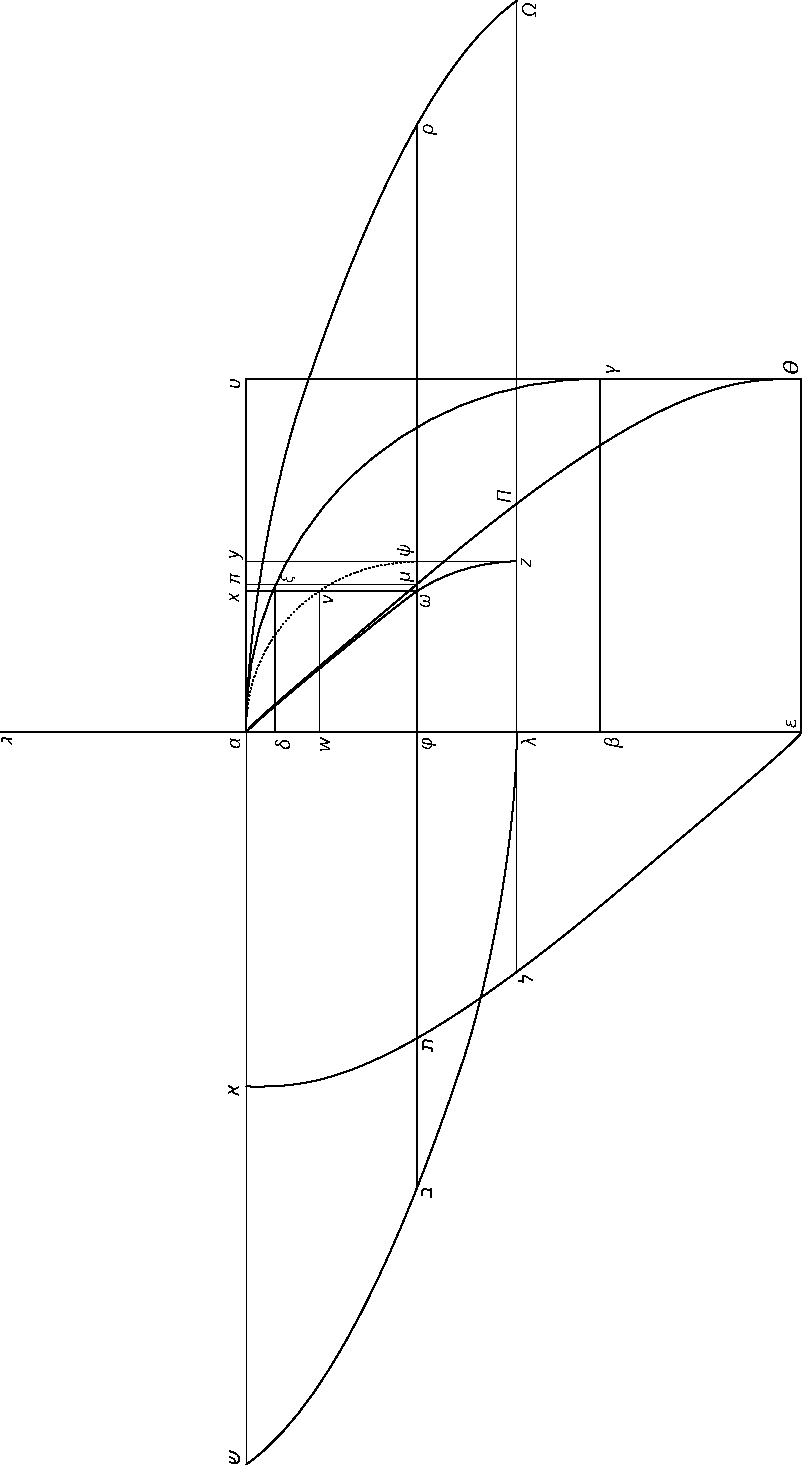
\includegraphics[width=0.66\textwidth]{gesamttex/edit_VIII,3/images/LH_35_09_15_012-013_d3a.pdf}}%
  \vspace{0.01em}%
  \centerline{\lbrack\textit{Fig.~3a}\rbrack}%
  \label{LH_35_09_15_013v_Fig.3}%
  \newpage% Rein vorläufig!
%
%
 % \vspace{0.5em}%
%  \newpage%  Rein vorläufig!
  \centerline{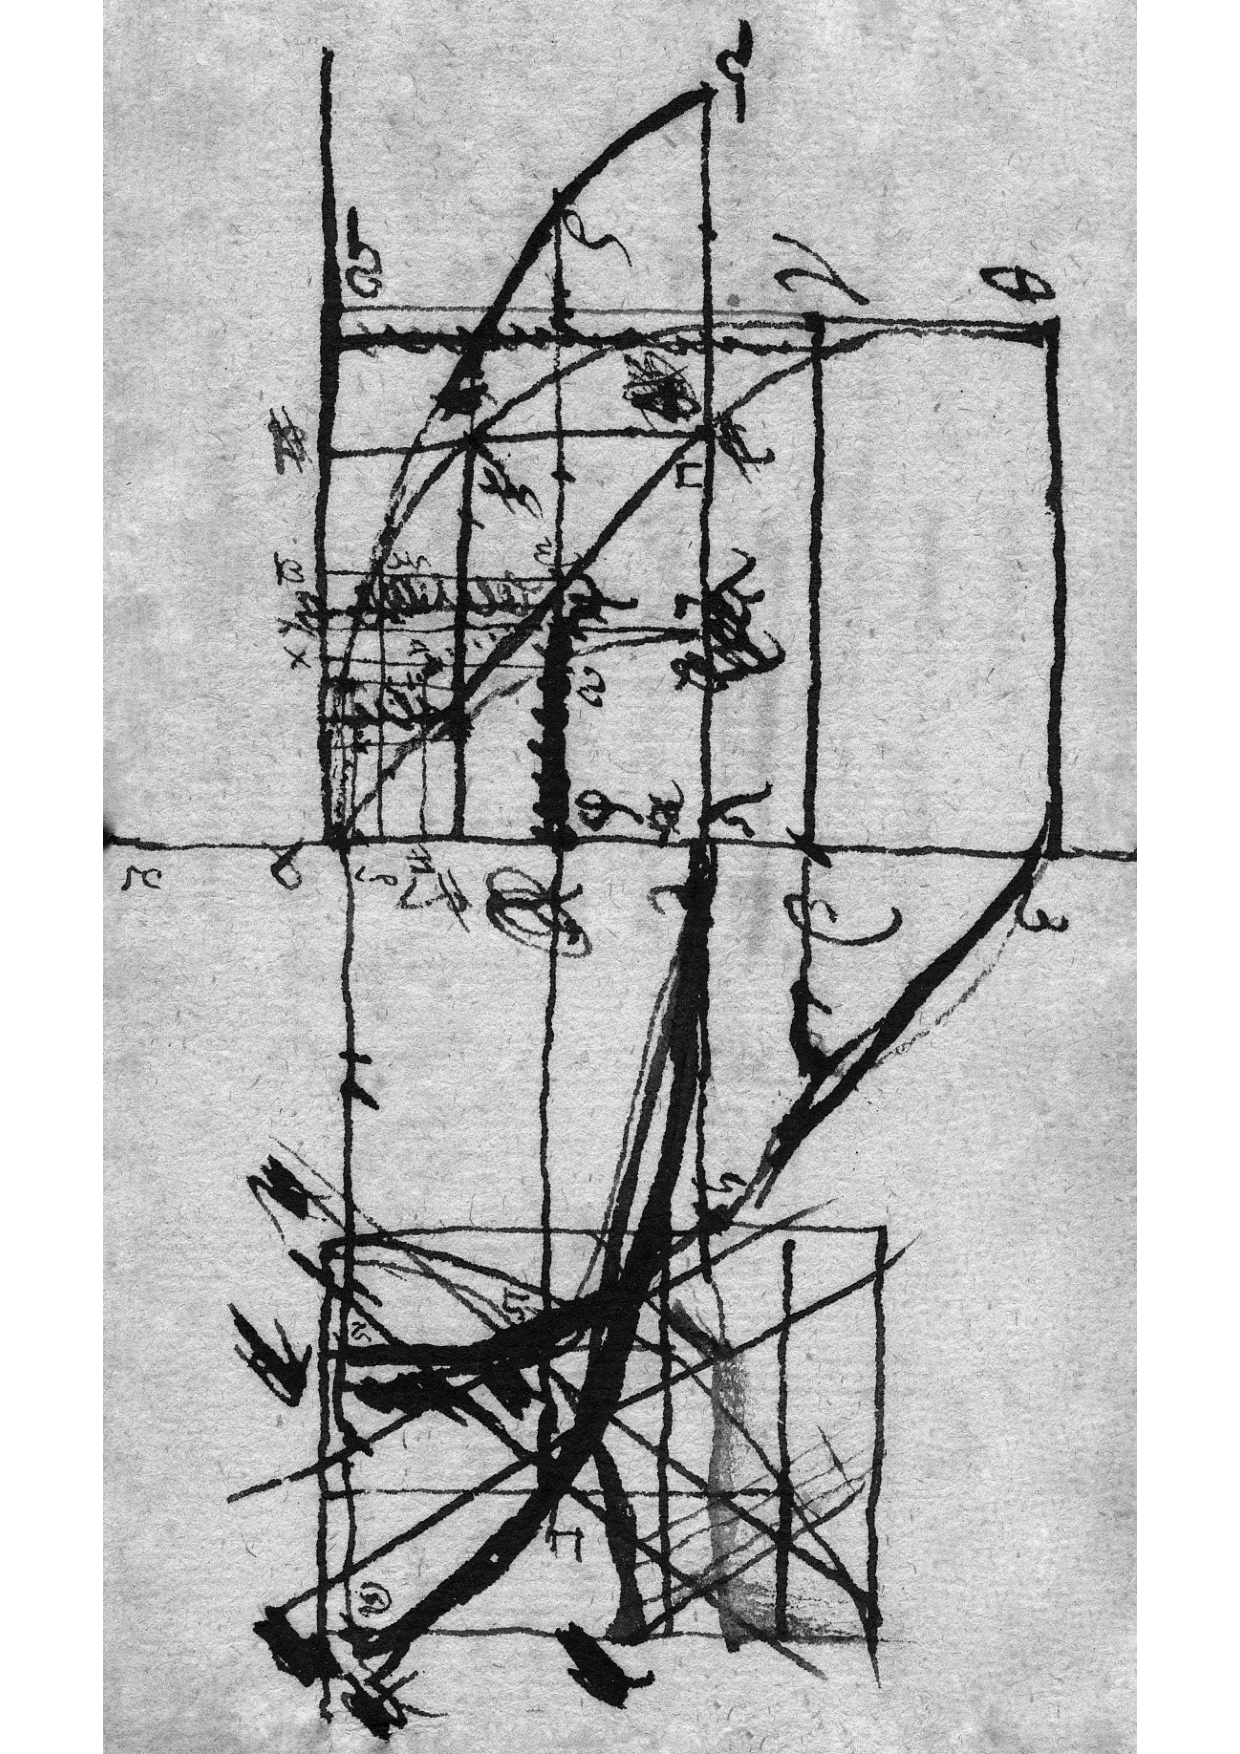
\includegraphics[width=0.835\textwidth]{gesamttex/edit_VIII,3/images/LH_35_09_15_012-013_d3b.pdf}}%\\
  \vspace{0.5em}
  \centerline{\lbrack\textit{Fig.~3b}\rbrack}%
  \label{LH_35_09_15_013v_Fig.3_fs}
%
%
% ENDE DES STÜCKES auf Blatt 13v
%
\newpage% REIN VORLÄUFIG !!!!!!
%